%$\{Y(t):t \geq 0\}$ is a birth and death process since whenever an indiv
%The continuous-time Markov chain is a birth and death process if the following is satisfied
%$$P_{i, i+1}(h) = \lambda_i + o(h) \text{ }(\text{as } h\rightarrow 0^+) \text{ for } i \geq 0$$
%$$P_{i, i-1}(h) = \mu_i + o(h) \text{ }(\text{as } h\rightarrow 0^+) \text{ for } i \geq 1$$
%$$P_{i, i+1}(h) = 1 - (\lambda_i + \mu_i)h+ o(h) \text{ }(\text{as } h\rightarrow 0^+) \text{ for } i \geq 0$$
%$$ P_{ij} = \delta_{ij} = 0 \text{ for } i \neq j $$
%$$ P_{ij} = \delta_{ij} = 1 \text{ for } i = j $$
%$$\mu_0 = 0, \lambda_0 > 0\text{ and } \mu_i, \lambda_i > 0 \text{ for } i\geq1.$$
%Alternative DEF:
%Whenever you jump to state i, two competing processes start: 
%$$\text{1) } T_1  = \text{ "time until birth" } \sim \text{ Exp}(\lambda_i)$$
%$$\text{2) } T_2 = \text{ "time until death" } \sim \text{ Exp}(\mu_i)$$
%The transition diagram for $\{Y(t): t\geq 0\}$ is illustrated in figure \ref{transdiagramY}.
\begin{figure}
    \centering
    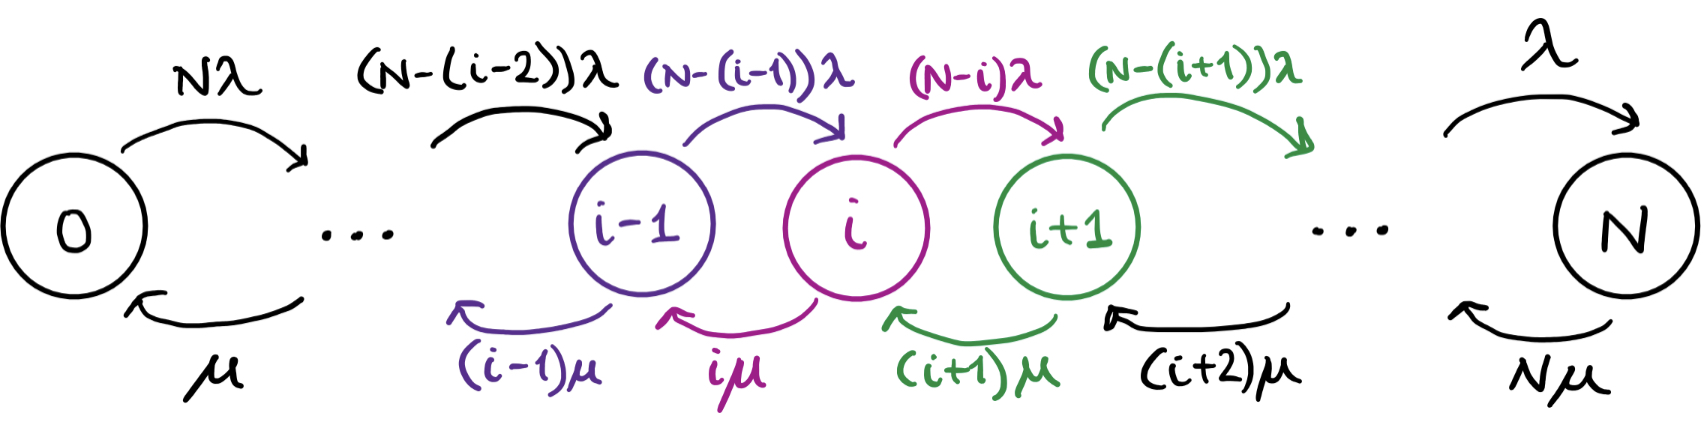
\includegraphics[width=140mm]{1f_new.png}
    \caption{Transition diagram of $\{Y(t):t \geq 0 \}$. $N$ is defined as the number of individual in a population, in this case $5.26 \text{ million.}$}
    \label{transdiagramY}
\end{figure}
%FORSLAG:
$\{Y(t):t \geq 0\}$ is a birth and death process because it in a given state $i$ only is possible to transition to either $i+1$ or $i-1$ and because the sojourn times are independent of each other. In each state there are two competing processes, which determine the next jump,
$$\text{1) } T_1  = \text{ "time until next infection" } \sim \text{ Exp}(\lambda_i)$$
$$\text{2) } T_2 = \text{ "time until next recovery" } \sim \text{ Exp}(\mu_i),$$
so that the sojourn time in state $i$ is $S_i \sim \text{ Exp}(\lambda_i +\mu_i)$.

As all individuals in the population become infected and susceptible completely independent of each other, the birth rate, i.e. the infection rate, will decrease as the number of susceptible individuals decreases. Correspondingly, the death or recovery rate will increase as the infected population increases. 

Let $\text{N}=5.26\text{million}$ be the total population size. Then the birth rate in state $i$ is given by $\lambda_i=(N-i)\lambda$ for $i=0,..,N$, where $\lambda$ is the transition rate from susceptible to infected for one individual. The death rate is similarly given by $\mu_i = i\mu$ for $i=0,...,N$, with $\mu$ the transition rate from infected to susceptible for one individual. This is illustrated in figure \ref{transdiagramY}.

